\documentclass{article}
\usepackage[UTF8]{ctex}
\usepackage[utf8]{inputenc} % allow utf-8 input
\usepackage[T1]{fontenc}    % use 8-bit T1 fonts
\usepackage{hyperref}       % hyperlinks
\usepackage{url}            % simple URL typesetting
\usepackage{booktabs}       % professional-quality tables
\usepackage{amsfonts}       % blackboard math symbols
\usepackage{nicefrac}       % compact symbols for 1/2, etc.
\usepackage{microtype}      % microtypography
\usepackage{lipsum}
\usepackage{geometry}
\usepackage{amssymb}
\usepackage{graphicx} %插入图片的宏包
\usepackage{float} %设置图片浮动位置的宏包
\usepackage{subfigure} %插入多图时用子图显示的宏包
\usepackage{listings}
\usepackage{soul}
\usepackage{tikz}
\usepackage{tikz-qtree}
\usepackage[colorlinks,linkcolor=blue]{hyperref}
\usepackage{tikz}
\usetikzlibrary{positioning, shapes.geometric}

\geometry{a4paper,scale=0.8}
\date{}

\usepackage{listings}
\usepackage{color}

\definecolor{dkgreen}{rgb}{0,0.6,0}
\definecolor{gray}{rgb}{0.5,0.5,0.5}
\definecolor{mauve}{rgb}{0.58,0,0.82}

\lstset{frame=tb,
  language=Python,
  aboveskip=3mm,
  belowskip=3mm,
  showstringspaces=false,
  columns=flexible,
  basicstyle={\small\ttfamily},
  numbers=none,
  numberstyle=\tiny\color{gray},
  keywordstyle=\color{blue},
  commentstyle=\color{dkgreen},
  stringstyle=\color{mauve},
  breaklines=true,
  breakatwhitespace=true,
  tabsize=3
}

\title{霍夫曼编码}


\author{
Huffman Coding\\
 刘卓\\
 \texttt{ } \\
}

\begin{document}
\maketitle

\section{定义}

\textit{\textbf{定义1}: 有根树(rooted tree )是指一个顶点(vertex)被指定为根的连通有向图(graph),它没有入边(edges),而其他顶点只有一条入边。}

~\\

\textbf{例1}:
$$
\begin{tikzpicture}[every tree node,
   level distance=1.25cm,sibling distance=1cm,
   edge from parent path={(\tikzparentnode) -- (\tikzchildnode)}]
\Tree [.\mbox{爷爷} [.\mbox{爸爸} [.\mbox{自己} ] [.\mbox{兄弟} ] ]]
\end{tikzpicture}
$$

$$
\begin{tikzpicture}[every tree node,
   level distance=1.25cm,sibling distance=1cm,
   edge from parent path={(\tikzparentnode) -- (\tikzchildnode)}]
\Tree [.${\color{red}\bullet}$	 [.${\color{red}\bullet}$ [.${\color{blue}\bullet}$ ] ] [.${\color{red}\bullet}$ [.${\color{red}\bullet}$ [.${\color{blue}\bullet}$ ] [.${\color{blue}\bullet}$ ] ] [.${\color{red}\bullet}$ [.${\color{blue}\bullet}$ ] ] [.${\color{blue}\bullet}$ ] [.${\color{blue}\bullet}$ ] ] [.${\color{blue}\bullet}$ ] ]
\end{tikzpicture}
$$

其中 ${\color{blue}\bullet}$ 为叶子(leaves),${\color{red}\bullet}$ 为内部顶点(internal vertex)。

$\hfill\square$ 

~\\

\textit{\textbf{定义2}: 二叉树(binary tree)是一棵有根的树,其中每个内部顶点不超过2个孩子(children)。全二叉树是一棵根树每个内部顶点都有两个孩子。}

~\\

\textbf{例2}:

不完全二叉树:

$$
\begin{tikzpicture}[every tree node,
   level distance=1.25cm,sibling distance=1cm,
   edge from parent path={(\tikzparentnode) -- (\tikzchildnode)}]
\Tree [.${\color{red}\bullet}$	
        [.${\color{red}\bullet}$ [.${\color{red}\bullet}$                                         [.${\color{blue}\bullet}$ ] [.${\color{blue}\bullet}$ ] ] ] 
        [.${\color{red}\bullet}$ [.${\color{blue}\bullet}$ ] [.${\color{red}\bullet}$             [.${\color{blue}\bullet}$ ] ] ] ]
\end{tikzpicture}
$$

完全二叉树:

$$
\begin{tikzpicture}[every tree node,
   level distance=1.25cm,sibling distance=1cm,
   edge from parent path={(\tikzparentnode) -- (\tikzchildnode)}]
\Tree [.${\color{red}\bullet}$  
        [.${\color{red}\bullet}$  [.${\color{red}\bullet}$  [.${\color{blue}\bullet}$ ]  [.${\color{blue}\bullet}$ ] ]  [.${\color{blue}\bullet}$ ] ] 
        [.${\color{red}\bullet}$  [.${\color{red}\bullet}$ [.${\color{blue}\bullet}$ ] [.${\color{blue}\bullet}$ ] ]  [.${\color{red}\bullet}$ [.${\color{blue}\bullet}$ ] [.${\color{blue}\bullet}$ ] ]  ]  ]
\end{tikzpicture}
$$

$\hfill\square$ 

~\\

\textit{\textbf{定义3}:如果两个码字的连接包含一个有效码字,且两者重叠,则这个二进制码字是无逗号(comma-free)}

~\\

\textbf{例3}:

令:
$$A = 000, B =001,C = 01 ,D = 10, E = 1100, F = 1101, G =111 $$

$$
\begin{tikzpicture}[every tree node,
   level distance=1.25cm,sibling distance=1cm,
   edge from parent path={(\tikzparentnode) -- (\tikzchildnode)}]
\Tree [.${\color{red}\bullet}$  \edge node[auto=right]{0}; 
        [.${\color{red}\bullet}$ \edge node[auto=right]{0};  [.${\color{red}\bullet}$ \edge node[auto=right]{0}; [.${\color{blue}A}$ ] \edge node[auto=left]{1};  [.${\color{blue}B}$ ] ]  \edge node[auto=left]{1};  [.${\color{blue}C}$ ] ] \edge node[auto=left]{1};
        [.${\color{red}\bullet}$  \edge node[auto=right]{0}; [.${\color{blue}D}$  ]  \edge node[auto=left]{1};  [.${\color{red}\bullet}$   \edge node[auto=right]{0}; [.${\color{red}\bullet}$ \edge node[auto=right]{0}; [.${\color{blue}E}$ ]  \edge node[auto=left]{1}; [.${\color{blue}F}$ ] ] \edge node[auto=left]{1}; [.${\color{blue}G}$ ] ]  ]  ]
        
\end{tikzpicture}
$$
$\hfill\square$ 

~\\

问:给定一个文件的字母频率,哪棵树需要最少的bit?

下面的算法给出了最优树:

\begin{enumerate}
\item 用一个节点/顶点替换每个字母,并根据每个字母的频率标记这些节点。然后,从左到右读取时,按节点值递增的顺序对节点进行排序。
\item 从左到右,把两个最小的数组合在一起,用它们的和代替它们。
\item 再次根据节点的值对结果节点进行排序。然后重复这些步骤,直到所有节点都连接好。
\item 一旦我们获得了二叉树,用相应的字母替换顶点数。然后我们把分支标记为左边是0,右边是1。
\item 最后,我们沿着路径跟踪以获得每个字母的代码。
\end{enumerate}

~\\

\textbf{例4}:
假设某个文件只包含以下频率的字母
$$
\begin{array}{|c|c|c|c|c|c|c|}
\hline \mathrm{A} & \mathrm{B} & \mathrm{C} & \mathrm{D} & \mathrm{E} & \mathrm{F} & \mathrm{G} \\
\hline 1 & 2 & 2 & 4 & 4 & 5 & 6 \\
\hline
\end{array}
$$

构造使您能够压缩文件的无逗号代码,以便您可以使用最少的位来存储它。

解:

第一步:

$$
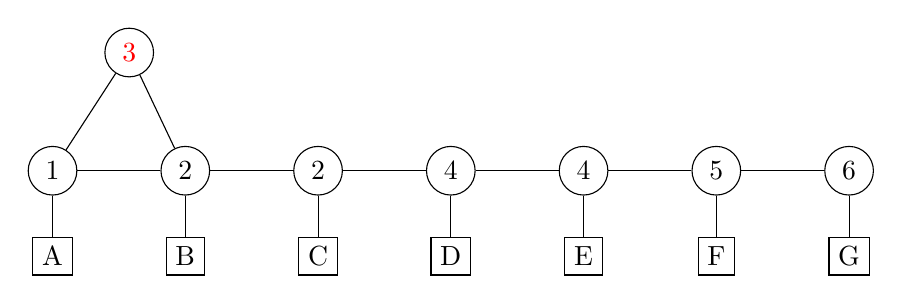
\begin{tikzpicture}[node distance=10pt]
  \node[draw, circle, aspect=2]     (A)  {1};
  \node[draw, circle, aspect=2, right=30pt of A]     (B)  {2};
  \node[draw, circle, aspect=2, right=30pt of B]     (C)  {2};
  \node[draw, circle, aspect=2, right=30pt of C]     (D)  {4};
  \node[draw, circle, aspect=2, right=30pt of D]     (E)  {4};
  \node[draw, circle, aspect=2, right=30pt of E]     (F)  {5};
  \node[draw, circle, aspect=2, right=30pt of F]     (G)  {6};
  \node[draw, aspect=2, below=15pt of A]     (A1)  {A};
  \node[draw, aspect=2, below=15pt of B]     (B1)  {B};
  \node[draw, aspect=2, below=15pt of C]     (C1)  {C};
  \node[draw, aspect=2, below=15pt of D]     (D1)  {D};
  \node[draw, aspect=2, below=15pt of E]     (E1)  {E};
  \node[draw, aspect=2, below=15pt of F]     (F1)  {F};
  \node[draw, aspect=2, below=15pt of G]     (G1)  {G};
  \node[draw, circle, aspect=2, above right=30pt and 15pt of A]  (A2)  {{\color{red}3}};
  
  \draw[-] (A) --  (B);
  \draw[-] (B) --  (C);
  \draw[-] (C) --  (D);
  \draw[-] (D) --  (E);
  \draw[-] (E) --  (F);
  \draw[-] (F) --  (G);
  \draw[-] (A) --  (A1);
  \draw[-] (B) --  (B1);
  \draw[-] (C) --  (C1);
  \draw[-] (D) --  (D1);
  \draw[-] (E) --  (E1);
  \draw[-] (F) --  (F1);
  \draw[-] (G) --  (G1);
  
  \draw[-] (A) --  (A2);
  \draw[-] (B) --  (A2);
\end{tikzpicture}
$$


第二步:

$$
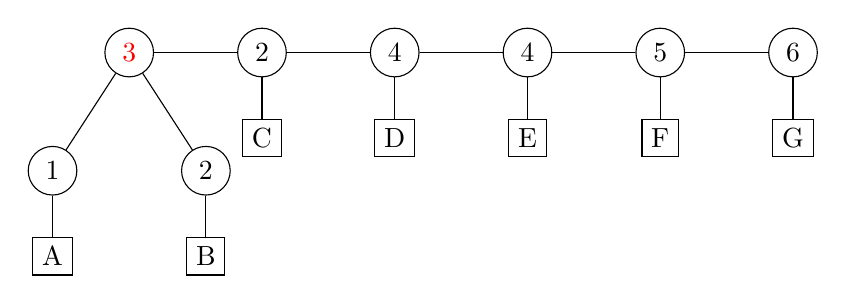
\begin{tikzpicture}[node distance=10pt]
  \node[draw, circle, aspect=2]  (A2)  {{\color{red}3}};
  \node[draw, circle, aspect=2,below left = 30pt and 15pt of A2]     (A)  {1};
  \node[draw, circle, aspect=2,below right = 30pt and 15pt of A2]     (B)  {2};
  \node[draw, circle, aspect=2, right=30pt of A2]     (C)  {2};
  \node[draw, circle, aspect=2, right=30pt of C]     (D)  {4};
  \node[draw, circle, aspect=2, right=30pt of D]     (E)  {4};
  \node[draw, circle, aspect=2, right=30pt of E]     (F)  {5};
  \node[draw, circle, aspect=2, right=30pt of F]     (G)  {6};
  \node[draw, aspect=2, below=15pt of A]     (A1)  {A};
  \node[draw, aspect=2, below=15pt of B]     (B1)  {B};
  \node[draw, aspect=2, below=15pt of C]     (C1)  {C};
  \node[draw, aspect=2, below=15pt of D]     (D1)  {D};
  \node[draw, aspect=2, below=15pt of E]     (E1)  {E};
  \node[draw, aspect=2, below=15pt of F]     (F1)  {F};
  \node[draw, aspect=2, below=15pt of G]     (G1)  {G};
  
  \draw[-] (A2) --  (C);
  \draw[-] (C) --  (D);
  \draw[-] (D) --  (E);
  \draw[-] (E) --  (F);
  \draw[-] (F) --  (G);
  \draw[-] (A) --  (A1);
  \draw[-] (B) --  (B1);
  \draw[-] (C) --  (C1);
  \draw[-] (D) --  (D1);
  \draw[-] (E) --  (E1);
  \draw[-] (F) --  (F1);
  \draw[-] (G) --  (G1);
  
  \draw[-] (A) --  (A2);
  \draw[-] (B) --  (A2);
\end{tikzpicture}
$$

第三步:

$$
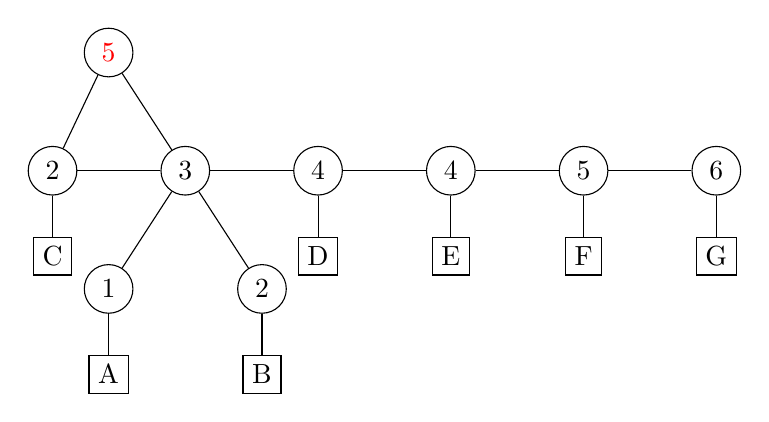
\begin{tikzpicture}[node distance=10pt]
  \node[draw, circle, aspect=2]  (A2)  {3};
  \node[draw, circle, aspect=2,below left = 30pt and 15pt of A2]     (A)  {1};
  \node[draw, circle, aspect=2,below right = 30pt and 15pt of A2]     (B)  {2};
  \node[draw, circle, aspect=2, left=30pt of A2]     (C)  {2};
  \node[draw, circle, aspect=2, right=30pt of A2]     (D)  {4};
  \node[draw, circle, aspect=2, right=30pt of D]     (E)  {4};
  \node[draw, circle, aspect=2, right=30pt of E]     (F)  {5};
  \node[draw, circle, aspect=2, right=30pt of F]     (G)  {6};
  \node[draw, aspect=2, below=15pt of A]     (A1)  {A};
  \node[draw, aspect=2, below=15pt of B]     (B1)  {B};
  \node[draw, aspect=2, below=15pt of C]     (C1)  {C};
  \node[draw, aspect=2, below=15pt of D]     (D1)  {D};
  \node[draw, aspect=2, below=15pt of E]     (E1)  {E};
  \node[draw, aspect=2, below=15pt of F]     (F1)  {F};
  \node[draw, aspect=2, below=15pt of G]     (G1)  {G};
  \node[draw, circle, aspect=2, above left = 30pt and 15pt of A2]     (F2)  {{\color{red}5}};

  \draw[-] (A2) --  (A);
  \draw[-] (A2) --  (B);
  \draw[-] (A2) --  (C);
  \draw[-] (A2) --  (F2);
  \draw[-] (A2) --  (D);
  \draw[-] (C) --  (F2);
  \draw[-] (D) --  (E);
  \draw[-] (E) --  (F);
  \draw[-] (F) --  (G);
  \draw[-] (A) --  (A1);
  \draw[-] (B) --  (B1);
  \draw[-] (C) --  (C1);
  \draw[-] (D) --  (D1);
  \draw[-] (E) --  (E1);
  \draw[-] (F) --  (F1);
  \draw[-] (G) --  (G1);
\end{tikzpicture}
$$

第四步:

$$
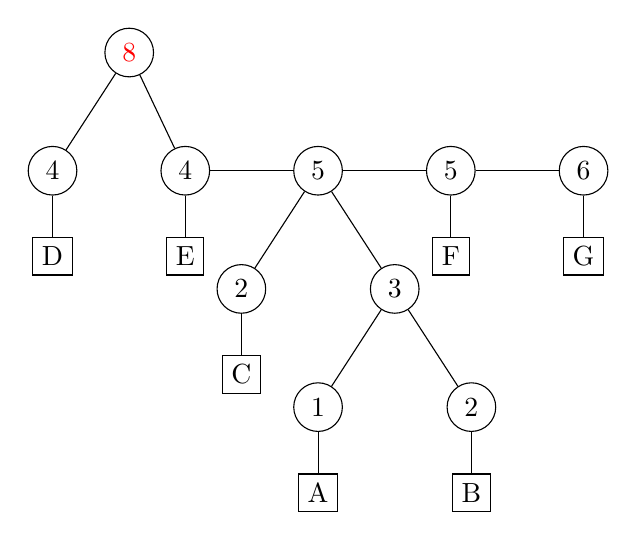
\begin{tikzpicture}[node distance=10pt]
  \node[draw, circle, aspect=2]     (F2)  {5};
  \node[draw, circle, aspect=2, ,below left = 30pt and 15pt of F2]     (C)  {2};
  \node[draw, circle, aspect=2,below right = 30pt and 15pt of F2]  (A2)  {3};
  \node[draw, circle, aspect=2,below left = 30pt and 15pt of A2]     (A)  {1};
  \node[draw, circle, aspect=2,below right = 30pt and 15pt of A2]     (B)  {2};
  \node[draw, circle, aspect=2, left=30pt of F2]     (E)  {4};
  \node[draw, circle, aspect=2, left =30pt of E]     (D)  {4};
  \node[draw, circle, aspect=2, right=30pt of F2]     (F)  {5};
  \node[draw, circle, aspect=2, right=30pt of F]     (G)  {6};
  \node[draw, aspect=2, below=15pt of A]     (A1)  {A};
  \node[draw, aspect=2, below=15pt of B]     (B1)  {B};
  \node[draw, aspect=2, below=15pt of C]     (C1)  {C};
  \node[draw, aspect=2, below=15pt of D]     (D1)  {D};
  \node[draw, aspect=2, below=15pt of E]     (E1)  {E};
  \node[draw, aspect=2, below=15pt of F]     (F1)  {F};
  \node[draw, aspect=2, below=15pt of G]     (G1)  {G};
  \node[draw, circle, aspect=2,above right = 30pt and 15pt of D]  (D2)  {{\color{red}8}};

  \draw[-] (A2) --  (A);
  \draw[-] (A2) --  (B);
  \draw[-] (A2) --  (F2);
  \draw[-] (C) --  (F2);
  \draw[-] (F) --  (G);
  \draw[-] (F) --  (F2);
  \draw[-] (F2) --  (E);
  \draw[-] (A) --  (A1);
  \draw[-] (B) --  (B1);
  \draw[-] (C) --  (C1);
  \draw[-] (D) --  (D1);
  \draw[-] (E) --  (E1);
  \draw[-] (F) --  (F1);
  \draw[-] (G) --  (G1);
  \draw[-] (D) --  (D2);
  \draw[-] (E) --  (D2);
\end{tikzpicture}
$$

第五步:

$$
\begin{tikzpicture}[node distance=10pt]
  \node[draw, circle, aspect=2]     (F2)  {5};
  \node[draw, circle, aspect=2,right = 30pt of G]  (D2)  {8};
  \node[draw, circle, aspect=2, ,below left = 30pt and 15pt of F2]     (C)  {2};
  \node[draw, circle, aspect=2,below right = 30pt and 15pt of F2]  (A2)  {3};
  \node[draw, circle, aspect=2,below left = 30pt and 15pt of A2]     (A)  {1};
  \node[draw, circle, aspect=2,below right = 30pt and 15pt of A2]     (B)  {2};
  \node[draw, circle, aspect=2, below  right=30pt and 15pt of D2]     (E)  {4};
  \node[draw, circle, aspect=2, below  left=30pt and 15pt of D2]     (D)  {4};
  \node[draw, circle, aspect=2, right=30pt of F2]     (F)  {5};
  \node[draw, circle, aspect=2, right=30pt of F]     (G)  {6};
  \node[draw, aspect=2, below=15pt of A]     (A1)  {A};
  \node[draw, aspect=2, below=15pt of B]     (B1)  {B};
  \node[draw, aspect=2, below=15pt of C]     (C1)  {C};
  \node[draw, aspect=2, below=15pt of D]     (D1)  {D};
  \node[draw, aspect=2, below=15pt of E]     (E1)  {E};
  \node[draw, aspect=2, below=15pt of F]     (F1)  {F};
  \node[draw, aspect=2, below=15pt of G]     (G1)  {G};
  \node[draw, circle, aspect=2,above right = 30pt and 15pt of F2]  (F3)  {{\color{red}10}};

  \draw[-] (A2) --  (A);
  \draw[-] (A2) --  (B);
  \draw[-] (A2) --  (F2);
  \draw[-] (C) --  (F2);
  \draw[-] (F) --  (G);
  \draw[-] (A) --  (A1);
  \draw[-] (B) --  (B1);
  \draw[-] (C) --  (C1);
  \draw[-] (D) --  (D1);
  \draw[-] (E) --  (E1);
  \draw[-] (F) --  (F1);
  \draw[-] (G) --  (G1);
  \draw[-] (G) --  (D2);
  \draw[-] (F3) --  (F2);
  \draw[-] (F3) --  (F);
  \draw[-] (D) --  (D2);
  \draw[-] (E) --  (D2);
\end{tikzpicture}
$$


第六步:

$$
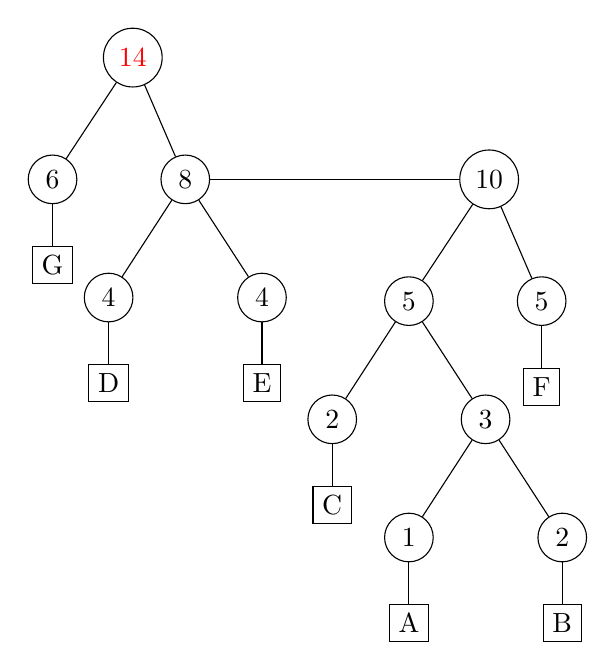
\begin{tikzpicture}[node distance=10pt]
  \node[draw, circle, aspect=2]  (F3)  {10};
  \node[draw, circle, aspect=2,below left = 30pt and 15pt of F3]     (F2)  {5};
  \node[draw, circle, aspect=2,left = 90pt of F3]  (D2)  {8};
  \node[draw, circle, aspect=2 ,below left = 30pt and 15pt of F2]     (C)  {2};
  \node[draw, circle, aspect=2,below right = 30pt and 15pt of F2]  (A2)  {3};
  \node[draw, circle, aspect=2,below left = 30pt and 15pt of A2]     (A)  {1};
  \node[draw, circle, aspect=2,below right = 30pt and 15pt of A2]     (B)  {2};
  \node[draw, circle, aspect=2, below  right=30pt and 15pt of D2]     (E)  {4};
  \node[draw, circle, aspect=2, below  left=30pt and 15pt of D2]     (D)  {4};
  \node[draw, circle, aspect=2, right=30pt of F2]     (F)  {5};
  \node[draw, circle, aspect=2, left=30pt of D2]     (G)  {6};
  \node[draw, aspect=2, below=15pt of A]     (A1)  {A};
  \node[draw, aspect=2, below=15pt of B]     (B1)  {B};
  \node[draw, aspect=2, below=15pt of C]     (C1)  {C};
  \node[draw, aspect=2, below=15pt of D]     (D1)  {D};
  \node[draw, aspect=2, below=15pt of E]     (E1)  {E};
  \node[draw, aspect=2, below=15pt of F]     (F1)  {F};
  \node[draw, aspect=2, below=15pt of G]     (G1)  {G};
  \node[draw, circle, aspect=2,above right = 30pt and 15pt of G]  (G2)  {{\color{red}14}};
  
  \draw[-] (A2) --  (A);
  \draw[-] (A2) --  (B);
  \draw[-] (A2) --  (F2);
  \draw[-] (C) --  (F2);
  \draw[-] (A) --  (A1);
  \draw[-] (B) --  (B1);
  \draw[-] (C) --  (C1);
  \draw[-] (D) --  (D1);
  \draw[-] (E) --  (E1);
  \draw[-] (F) --  (F1);
  \draw[-] (G) --  (G1);
  \draw[-] (F3) --  (F2);
  \draw[-] (F3) --  (F);
  \draw[-] (D) --  (D2);
  \draw[-] (E) --  (D2);
  \draw[-] (G) --  (G2);
  \draw[-] (D2) --  (G2);
  \draw[-] (D2) --  (F3);
\end{tikzpicture}
$$

第七步:

$$
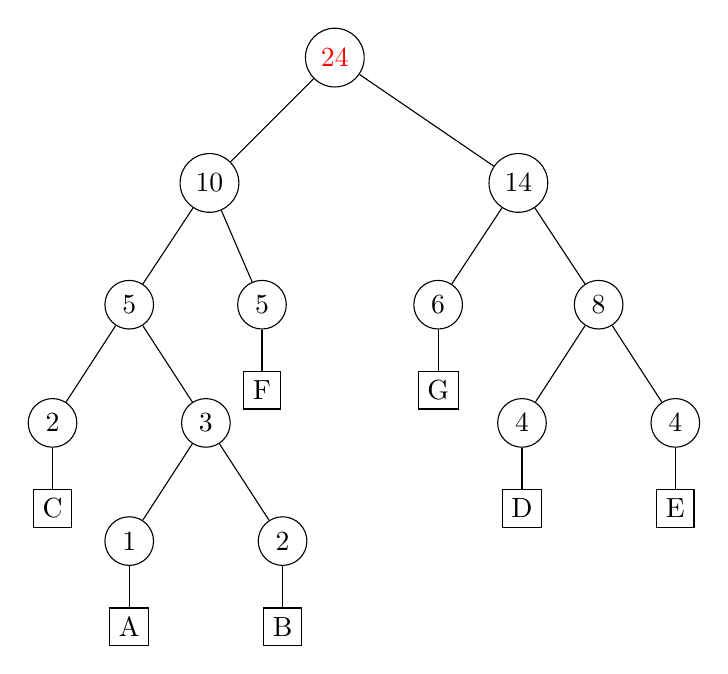
\begin{tikzpicture}[node distance=10pt]
  \node[draw, circle, aspect=2]  (F3)  {10};
  \node[draw, circle, aspect=2, right = 90pt of F3]  (G2)  {14};
  \node[draw, circle, aspect=2,below left = 30pt and 15pt of F3]     (F2)  {5};
  \node[draw, circle, aspect=2,below  right=30pt and 15pt of G2]  (D2)  {8};
  \node[draw, circle, aspect=2 ,below left = 30pt and 15pt of F2]     (C)  {2};
  \node[draw, circle, aspect=2,below right = 30pt and 15pt of F2]  (A2)  {3};
  \node[draw, circle, aspect=2,below left = 30pt and 15pt of A2]     (A)  {1};
  \node[draw, circle, aspect=2,below right = 30pt and 15pt of A2]     (B)  {2};
  \node[draw, circle, aspect=2, below  right=30pt and 15pt of D2]     (E)  {4};
  \node[draw, circle, aspect=2, below  left=30pt and 15pt of D2]     (D)  {4};
  \node[draw, circle, aspect=2, right=30pt of F2]     (F)  {5};
  \node[draw, circle, aspect=2,below  left=30pt and 15pt of G2]     (G)  {6};
  \node[draw, aspect=2, below=15pt of A]     (A1)  {A};
  \node[draw, aspect=2, below=15pt of B]     (B1)  {B};
  \node[draw, aspect=2, below=15pt of C]     (C1)  {C};
  \node[draw, aspect=2, below=15pt of D]     (D1)  {D};
  \node[draw, aspect=2, below=15pt of E]     (E1)  {E};
  \node[draw, aspect=2, below=15pt of F]     (F1)  {F};
  \node[draw, aspect=2, below=15pt of G]     (G1)  {G};
    \node[draw, circle, aspect=2,above right = 30pt and 30pt of F3]     (F5)  {{\color{red}24}};

  
  \draw[-] (A2) --  (A);
  \draw[-] (A2) --  (B);
  \draw[-] (A2) --  (F2);
  \draw[-] (C) --  (F2);
  \draw[-] (A) --  (A1);
  \draw[-] (B) --  (B1);
  \draw[-] (C) --  (C1);
  \draw[-] (D) --  (D1);
  \draw[-] (E) --  (E1);
  \draw[-] (F) --  (F1);
  \draw[-] (G) --  (G1);
  \draw[-] (F3) --  (F2);
  \draw[-] (F3) --  (F);
  \draw[-] (D) --  (D2);
  \draw[-] (E) --  (D2);
  \draw[-] (G) --  (G2);
  \draw[-] (D2) --  (G2);
  \draw[-] (F3) --  (F5);
  \draw[-] (G2) --  (F5);
\end{tikzpicture}
$$

可转化为:

$$
\begin{tikzpicture}[every tree node,
   level distance=1.25cm,sibling distance=1cm,
   edge from parent path={(\tikzparentnode) -- (\tikzchildnode)}]
\Tree [.${\color{red}\bullet}$  \edge node[auto=right]{0}; 
            [.${\color{red}\bullet}$ \edge node[auto=right]{0};  [.${\color{red}\bullet}$ \edge node[auto=right]{0}; [.${\color{blue}C}$ ] \edge node[auto=left]{1};                                                                                                                                                                           [.${\color{red}\bullet}$ \edge node[auto=right]{0}; [.${\color{blue}A}$ ] \edge node[auto=left]{1}; [.${\color{blue}B}$ ] ] ]  \edge node[auto=left]{1};                                                                                                                      [.${\color{blue}F}$ ] ] \edge node[auto=left]{1};
            [.${\color{red}\bullet}$  \edge node[auto=right]{0}; [.${\color{blue}G}$  ]  \edge node[auto=left]{1};                                                                                        [.${\color{red}\bullet}$   \edge node[auto=right]{0}; [.${\color{blue}G}$ ] \edge                                                                                         node[auto=left]{1}; [.${\color{blue}E}$ ] ]  ]  ]
        
\end{tikzpicture}
$$

$$
\begin{array}{|c|c|c|c|c|c|c|c|}
\hline \text { \mbox{字母} } & \mathrm{A} & \mathrm{B} & \mathrm{C} & \mathrm{D} & \mathrm{E} & \mathrm{F} & \mathrm{G} \\
\hline \text { \mbox{频率} } & 1 & 2 & 2 & 4 & 4 & 5 & 6 \\
\hline \text { Code } & 0010 & 0011 & 000 & 110 & 111 & 01 & 10 \\
\hline \text { Bits } & 4 & 4 & 3 & 3 & 3 & 2 & 2 \\
\hline
\end{array}
$$

因此加密后的长度为
$$4N_A+4N_B+3N_C+3N_D+3N_E+2N_F+2N_G = 64$$

因此相比未加密前的字符,平均每个字符需要$\frac{\mbox{密文长度}}{\mbox{明文长度}}\frac{64}{24} \approx 2.66$个bit替代

其熵值为:

\begin{eqnarray}   
\label{eq}
\sum_{\alpha} \mathbb{P}(\alpha) \log _{2}\left(\frac{1}{\mathbb{P}(\alpha)}\right)&=& \frac{1}{24} \log _{2}\left(\frac{1}{1 / 24}\right)+\frac{2}{24} \log _{2}\left(\frac{1}{2 / 24}\right)+\frac{2}{24} \log _{2}\left(\frac{2}{1 / 24}\right) \nonumber \\ 
&+&\frac{4}{24} \log _{2}\left(\frac{1}{4 / 24}\right)+\frac{4}{24} \log _{2}\left(\frac{1}{4 / 24}\right) \nonumber \\
&+& \frac{5}{24} \log _{2}\left(\frac{1}{5 / 24}\right)+\frac{6}{24} \log _{2}\left(\frac{1}{6 / 24}\right)  \nonumber \\
&\approx & 2.62165 \nonumber \\
\nonumber 
\end{eqnarray}

$\hfill\square$ 

\textit{\textbf{定理1}: 假设明文中的字母数为$n_1,n_2,\cdots,n_k$,且设$N = n_1 + \cdots+ n_k$。那么最佳代码长度(以每个字母的比特数表示)是
}
$$H = \sum_{i = 1}^{k}p_i \log_2\left( \frac{1}{p_i} \right) $$

\textit{其中$p_i = n_i / N $, $1 \leq i \leq k$。
}

\textit{\textbf{定理2}:由概率$p_1, p_2, \cdots,p_k$产生的预期码长在熵的1 bit以内}
$$H = \sum_{i = 1}^{k}p_i \log_2\left( \frac{1}{p_i} \right) $$
\textit{其中$p_i = n_i / N $, $1 \leq i \leq k$。
}


\textit{\textbf{定理3:}仅针对密文攻击}
$$H(K|C) = H(K)+H(M)-H(C)$$

\textit{\textbf{定理4:}仅针对明文攻击}
$$H(K|C,M) = H(K)+H(C|M)$$

\section{随机密码系统}

设计:

\begin{itemize}
\item 明文$M = {m_1,m_2,\cdots,m_N}$
\item 密钥$K = {k_1,k_2,\cdots,k_S}$
\item 密文$C = {c_1,c_2,\cdots,c_Q}$
\item 使用密钥k的加密公式:$c = E_k(m)$
\item 使用密钥k的解密公式:$m = D_k(c)$
\end{itemize}

\textbf{例5}

明文:$m_1,m_2,m_3$

密钥:$k_1,k_2,k_3,k_4$

密文:$c_1,c_2,c_3,c_4$

$$
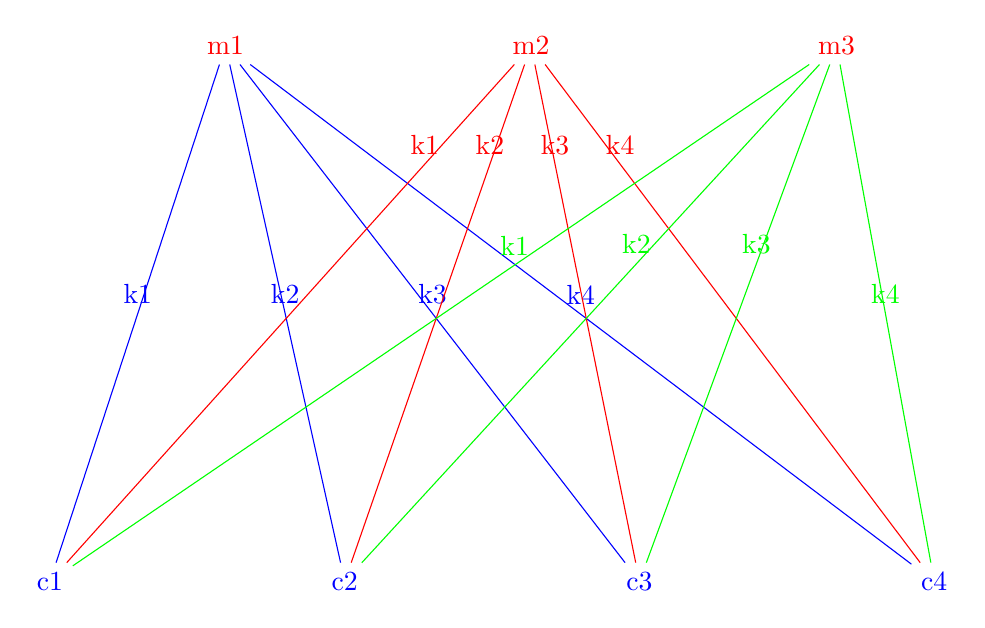
\begin{tikzpicture}[node distance=10pt]
  \node[]  (m1)  {{\color{red}m1}};
  \node[right = 90pt of m1]  (m2)  {{\color{red}m2}};
  \node[right = 90pt of m2]  (m3)  {{\color{red}m3}};
  \node[below left = 180pt and 45pt of m1]  (c1)  {{\color{blue}c1}};
  \node[right = 90pt of c1]  (c2)  {{\color{blue}c2}};
  \node[right = 90pt of c2]  (c3)  {{\color{blue}c3}};
  \node[right = 90pt of c3]  (c4)  {{\color{blue}c4}};

  \draw[blue,-] (m1) -- node[blue,above]  {k1} (c1);
  \draw[blue,-] (m1) -- node[blue,above]  {k2} (c2);
  \draw[blue,-] (m1) -- node[blue,above]  {k3} (c3);
  \draw[blue,-] (m1) -- node[blue,above]  {k4} (c4);
  \draw[red,-] (m2) -- node[red,above,pos=0.2]  {k1} (c1);
  \draw[red,-] (m2) -- node[red,above,pos=0.2]  {k2} (c2);
  \draw[red,-] (m2) -- node[red,above,pos=0.2]  {k3} (c3);
  \draw[red,-] (m2) -- node[red,above,pos=0.2]  {k4} (c4);
  \draw[green,-] (m3) -- node[green,above,pos=0.4]  {k1} (c1);
  \draw[green,-] (m3) -- node[green,above,pos=0.4]  {k2} (c2);
  \draw[green,-] (m3) -- node[green,above,pos=0.4]  {k3} (c3);
  \draw[green,-] (m3) -- node[green,above]  {k4} (c4);
\end{tikzpicture}
$$


由此可知,一个密文,可能对应三种明文,破解难度加大。

$\hfill\square$ 

\section{完善保密性Perfect Secrecy}

\textit{\textbf{定义4}:如果密文不提供关于明文的信息,就说密码系统达到完全保密。即M、C为随机变量,即}
$$
\mathbb{P}\left(M=m_{i} \cap C=c_{j}\right)=\mathbb{P}\left(M=m_{i}\right) \cdot \mathbb{P}\left(C=c_{j}\right)
$$

其中$m_j \in M$, $c_j\in C$。

因此在一个完善的保密系统中:

\begin{itemize}
\item 密钥的数量至少必须与密文的数量一样大。
\item 对于固定密钥:不同的明文对应不同的密文。因此,密文的数量必须至少与明文的数量相等。
\end{itemize}

即:密钥数量 $\ge$ 密文数量 $\ge$ 明文数量

~\\

\textit{\textbf{定理5:}完全保密应该满足于:
\begin{itemize}
\item 所有密钥概率应该相等
\item 对于加密过程$m_i$到$c_i$,都为唯一的密钥k与之对应
\end{itemize}
}

那么如果建立的一个完善的保密方法呢?需要有以下几点要求:

\begin{itemize}
\item 密钥数量 = 密文数量 = 明文数量
\item 所有密钥概率应该相等
\item 加密矩阵是拉丁方图(Latin square )或加密图是完全二部图(complete
bipartite graph)。
    \begin{itemize}
    \item 拉丁方图是一个$n \times n$矩阵,其中整数从1到n在每一行和每一列中只出现一次。
    \item 完全二部图是一个图,它的顶点集合被分解成两个不相交的子集,使得同一个子集中的两个顶点不连通,且每个顶点之间有一条边
\end{itemize}
\end{itemize}

\textbf{例6}

明文:$m_1,m_2,m_3$

密钥:$k_1,k_2,k_3$

密文:$c_1,c_2,c_3$

拉丁方图:
$$
\begin{array}{l|lll} 
& m_{1} & m_{2} & m_{3} \\
\hline k_{1} & c_{1} & c_{2} & c_{3} \\
k_{2} & c_{2} & c_{3} & c_{1} \\
k_{3} & c_{3} & c_{1} & c_{2}
\end{array}
$$

完全二部图:

$$
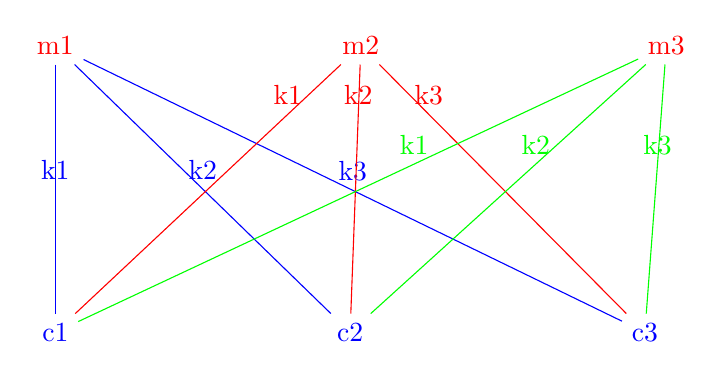
\begin{tikzpicture}[node distance=10pt]
  \node[]  (m1)  {{\color{red}m1}};
  \node[right = 90pt of m1]  (m2)  {{\color{red}m2}};
  \node[right = 90pt of m2]  (m3)  {{\color{red}m3}};
  \node[below = 90pt of m1]  (c1)  {{\color{blue}c1}};
  \node[right = 90pt of c1]  (c2)  {{\color{blue}c2}};
  \node[right = 90pt of c2]  (c3)  {{\color{blue}c3}};

  \draw[blue,-] (m1) -- node[blue,above]  {k1} (c1);
  \draw[blue,-] (m1) -- node[blue,above]  {k2} (c2);
  \draw[blue,-] (m1) -- node[blue,above]  {k3} (c3);
  \draw[red,-] (m2) -- node[red,above,pos=0.2]  {k1} (c1);
  \draw[red,-] (m2) -- node[red,above,pos=0.2]  {k2} (c2);
  \draw[red,-] (m2) -- node[red,above,pos=0.2]  {k3} (c3);
  \draw[green,-] (m3) -- node[green,above,pos=0.4]  {k1} (c1);
  \draw[green,-] (m3) -- node[green,above,pos=0.4]  {k2} (c2);
  \draw[green,-] (m3) -- node[green,above,pos=0.4]  {k3} (c3);
\end{tikzpicture}
$$








\end{document}

